\chapter{Numerical Experiments}
\label{cha:3}
In this chapter we shall compare the augmented Lagrangian Method with several industry standard backpropagation algorithms. We considered the following algorithms: ADAM, ...

The first comparison will be run on a small example, for which we expect that all algorithms should easily converge to a good solution.

\section{Training Algorithms and Stopping Criteria}
This section will discuss the problem of comparing different training algorithms, which is not as straightforward as it might seem. In the literature many different methods of comparison are used. The main issue is the choice of stopping criterion. One could choose a tolerance for the loss function, but this is dependent on the problem at hand, and it is not possible to know beforehand what a "low" cost is for the selected network. Another option is to select a set number of epochs, but epochs of one algorithm are not necessarily equivalent to epochs of another algorithm. Finally the most straightforward option would be to let each algorithm run for a specified amount of time, and compare the loss on the training set after each run. In a certain way this might be the most fair option, because average running time is the most important factor in practice, if the final performance is similar. On the other hand it is hard for a new, experimental method to be as optimally coded as one that has been used in the field for many years already.

In practice in machine learning usually early stopping criteria are used, to protect against overfitting. The most common early stopping criterion is to stop when a minimum in the validation dataset has been reached. Further complicating matters is that because of the complexity of the loss surface of a DNN, and the random initialization of the weight matrices, each optimization run will follow a completely different trajectory and find a different local minimum.

Because the goal of this thesis is in the first place to compare training performance, overfitting is not of great concern. Therefore no validation data will be used in the training process. Instead the training will stop once a minimum in the training performance has been reached, indicated by a stagnation in the improvement in training performance.

For these reasons ALM will stop when the following inequality holds true:

\begin{equation}
(1+\epsilon)C(W_{k+1}) > C(W_k)
\end{equation}

Where $C(W_k)$ is the loss at epoch $k$ and $\epsilon$ is a small tolerance value. Because ALM only takes only few, but comparatively costly, epochs to converge, it should make sense to not wait many epochs to confirm that the algorithm has reached a minimum. This stopping criteria is similar to the one proposed by the original paper for Algorithm \ref{algo} \cite{sahin2019}, in that it is also in some sense a limit to the gradient of \ref{loss}. However the influence of the state variables and the constraint violations have been discarded.

The algorithm against which the ALM method will be compared is the ADAM algorithm, which may take thousands of epochs to converge. To find the minimum in the training loss the \texttt{EarlyStopping} method implemented in \texttt{tensorflow.keras} will be used. This method has a patience value $p$, meaning that the training will stop once $p$ epochs have passed without any improvement.
 

\section{Test setup}
Each test will average the results over many training runs so as to get a more accurate and fair picture of the performance that can be expected from each algorithm. Typically each test will use 20 training runs.

The training performance of ALM will be compared to the ADaptive Moment Estimation (ADAM) optimizer, which is a type of Stochastic Gradient Descent (SGD) method. This optimizer is widely used and is generally known to be robust (Goodfellow et al. \cite{Goodfellow-et-al-2016}, Sec. 8.5.3). Even though it is usually used in a mini-batch manner, the datasets in these problems are so small that the batch size is set to be as large as the dataset. This effectively makes it a true Gradient Descent method instead of an SGD. The learning rate is left at the default $0.001$. 

The weights of the network will be initialized using Xavier initialization for layers using the $\tanh(x)$ activation function and Kaiming initialization for layers using the ReLU activation function. Both training algorithms will start from the same initial point for each test. ADAM will halt when 10 epochs have passed without improvement, indicating a local minimum has been reached. For ALM the training will halt after a single epoch has passed without significant improvement:

\begin{equation}
(1+\epsilon)F(u_{k+1}) > F(u_k)
\end{equation}

Where $F(u_k)$ is the loss at epoch $k$ and $\epsilon$ is chosen to be $1e^{-2}$.

All tests are run on Intel(R) Core(TM) i5-7300HQ CPU @ 2.50GHz with 8Gi RAM and SSD hard disk. 

\section{Fully connected feedforward network}
For the first comparison a similar regression problem as in Chapter 2 will be considered. The sine function in equation \ref{sin} is quite simple, therefore a problem with a more depth is considered: a squared sine function. The function definition is as follows: 

\begin{equation}
y = \sin^2(x) + \mathcal N(0,\delta), x \in [0,\pi]
\label{sin2}
\end{equation}

\begin{figure}[p]
     \centering
     \begin{subfigure}[b]{0.49\textwidth}
         \centering
         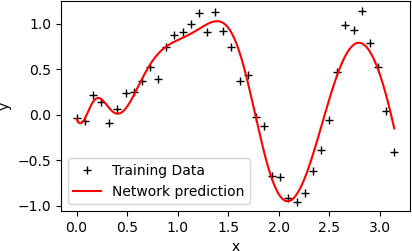
\includegraphics[width=\textwidth]{almgood}
         \caption{Example of good convergence}
         \label{almgood}
     \end{subfigure}
     \begin{subfigure}[b]{0.49\textwidth}
         \centering
         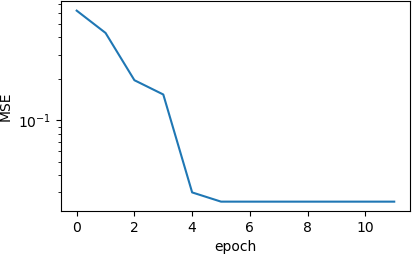
\includegraphics[width=\textwidth]{almgoodconv}
         \caption{Training history of convergence}
         \label{almgoodconv}
     \end{subfigure}
     \caption{Example of convergence behaviour of ALM optimizer for network using $tanh$ activation and 40 data points. The network has 2 hidden layers of 8 nodes. An example of bad convergence could not be found for the $tanh$ activation function using ALM.}
     \label{almconv}
\end{figure}

\begin{figure}[p]
     \begin{subfigure}[b]{0.49\textwidth}
         \centering
         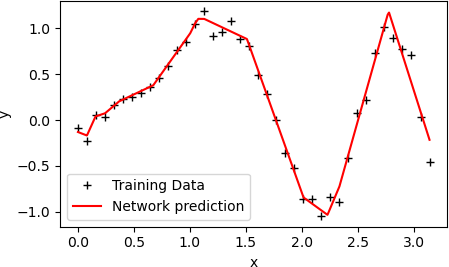
\includegraphics[width=\textwidth]{adamgood}
         \caption{Example of good convergence}
         \label{adamgood}
     \end{subfigure}
     \begin{subfigure}[b]{0.49\textwidth}
         \centering
         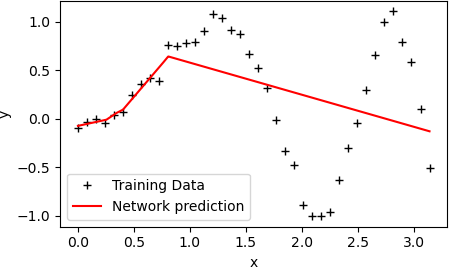
\includegraphics[width=\textwidth]{adambad}
         \caption{Example of bad convergence}
         \label{adambad}
     \end{subfigure}
     \begin{subfigure}[b]{0.49\textwidth}
         \centering
         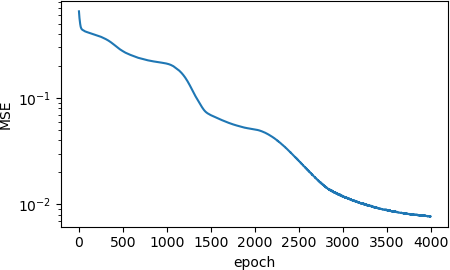
\includegraphics[width=\textwidth]{adamgoodconv}
         \caption{Training history of good convergence}
         \label{adamgoodconv}
     \end{subfigure}
     \begin{subfigure}[b]{0.49\textwidth}
         \centering
         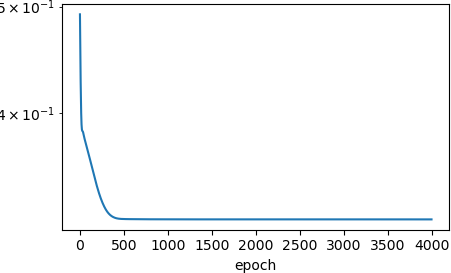
\includegraphics[width=\textwidth]{adambadconv}
         \caption{Training history of bad convergence}
         \label{adambadconv}
     \end{subfigure}
    \caption{Examples of convergence behaviour of ADAM optimizer for network using ReLU activation and 40 data points. The network has 2 hidden layers of 16 nodes.}
    \label{adamconv}
\end{figure}

This function oscillates progressively faster, and the training algorithm will not always find a good solution. Figure \ref{adamconv} shows two examples runs of the ADAM optimizer for 4000 epochs. The only difference is the choice of initial weights and the random noise. The first example has converged well, and would probably improve even further if the number of epochs was increased. The second example has stagnated in a bad minimum. Figure \ref{almconv} shows an example run of the ALM optimizer for 12 epochs using the $tanh$ activation function. An example of bad convergence using this activation could not be found.

For the first experiment two similar networks are trained to approximate function \ref{sin2}. The first network has 2 hidden layers of 8 nodes with $tanh$ activation function, the second has 2 hidden layers of 16 nodes with a ReLU activation function. Each is trained with progressively more data points. Every single configuration is run 20 times. The results are listed in table \ref{restab}. The code from this test is found in appendix \ref{app:B}

\begin{table}
\renewcommand{\arraystretch}{1.3}
\centering
\footnotesize
\makebox[\textwidth][c]{
\begin{tabular}{r | r| c c c c c || r| c c c c c|}
\multicolumn{1}{c}{} & \multicolumn{6}{c}{$\sigma(\cdot) = \tanh(\cdot)$} & 
                       \multicolumn{6}{c}{$\sigma(\cdot) = \max(\cdot,0)$} \\\cline{2-13}
%    ADAM& \multirow{2}{*}{10} & $1.28e^{-2} $ & $ 1.56e^{-12}$ & $ 120 $ & $ 926 $ & $ 19 $ & \multirow{2}{*}{20} & $3.73e^{-2} $ & $ 2.89e^{-4} $ & $ 41.0 $ & $ 351 $  & $ 12$ \\
%    ALM & 				      & $3.77e^{-2} $ & $ 9.05e^{-3} $ & $ 1.39$ & $ 6.40$ & $ 20 $ & 				      & $8.48e^{-2} $ & $ 4.97e^{-4} $ & $ 2.52 $ & $ 6.47 $ & $ 17$ \\ \cline{2-13}
%    ADAM& \multirow{2}{*}{20} & $4.44e^{-3} $ & $ 6.90e^{-4} $ & $ 117 $ & $ 878 $ & $ 16 $ & \multirow{2}{*}{40} & $6.34e^{-2} $ & $ 8.51e^{-3} $ & $ 53.0 $ & $ 478 $  & $ 9 $ \\
%    ALM & 					  & $1.07e^{-1} $ & $ 4.40e^{-3} $ & $ 8.29$ & $ 7.47$ & $ 19 $ & 					  & $9.85e^{-2} $ & $ 6.99e^{-3} $ & $ 8.69 $ & $ 5.42 $ & $ 12 $\\ \cline{2-13}
%    ADAM& \multirow{2}{*}{40} & $8.49e^{-3} $ & $ 7.54e^{-3} $ & $ 118 $ & $ 939 $ & $ 15 $ & \multirow{2}{*}{80} & $6.55e^{-2} $ & $ 4.14e^{-2} $ & $ 38.8 $ & $ 352 $  & $ 10 $\\
%    ALM &                     & $2.22e^{-2} $ & $ 8.56e^{-3} $ & $ 7.94$ & $ 7.05$ & $ 20 $ &                     & $9.23e^{-2} $ & $ 2.24e^{-2} $ & $ 14.2 $ & $ 4.12 $ & $ 17 $\\ \cline{2-13}

        &                   N & avg MSE       & best MSE        & time(s)  & epochs   & conv   &                   N & avg MSE        & best MSE       & time(s)  & epochs   & conv   \\ \cline{2-13}
    ADAM& \multirow{2}{*}{10} & $ 2.09e^{-2} $ & $1.20e^{-11} $ & $ 18.7 $ & $ 3790 $ & $ 17 $ & \multirow{2}{*}{20} & $ 1.22e^{-1} $ & $ 3.15e^{-3} $ & $ 30.3 $ & $ 3500 $ & $ 5  $ \\
    ALM & 				      & $ 2.10e^{-1} $ & $ 1.59e^{-1} $ & $ 1.85 $ & $ 6.38 $ & $ 16 $ & 				     & $ 1.63e^{-1} $ & $ 1.08e^{-2} $ & $ 4.41 $ & $ 5.47 $ & $ 15 $ \\ \cline{2-13}
    ADAM& \multirow{2}{*}{20} & $ 1.25e^{-2} $ & $ 9.84e^{-4} $ & $ 19.8 $ & $ 3960 $ & $ 17 $ & \multirow{2}{*}{40} & $ 6.28e^{-2} $ & $ 8.85e^{-3} $ & $ 22.4 $ & $ 2690 $ & $ 5  $ \\
    ALM & 					  & $ 5.87e^{-2} $ & $ 7.69e^{-3} $ & $ 8.06 $ & $ 7.50 $ & $ 20 $ & 					 & $ 9.89e^{-2} $ & $ 1.37e^{-2} $ & $ 8.09 $ & $ 5.11 $ & $ 18 $ \\ \cline{2-13}
    ADAM& \multirow{2}{*}{40} & $ 2.56e^{-2} $ & $ 7.58e^{-3} $ & $ 19.2 $ & $ 3920 $ & $ 15 $ & \multirow{2}{*}{80} & $ 7.61e^{-2} $ & $ 7.64e^{-3} $ & $ 29.9 $ & $ 3150 $ & $ 4  $ \\
    ALM &                     & $ 1.61e^{-2} $ & $ 7.90e^{-3} $ & $ 11.6 $ & $ 6.90 $ & $ 20 $ &                     & $ 1.02e^{-1} $ & $ 1.03e^{-2} $ & $ 25.3 $ & $ 4.21 $ & $ 14 $ \\ \cline{2-13}


\end{tabular}
}
\caption{Results of tests using $\tanh$ and ReLU activation function.}
\label{restab}

\end{table}

The last column of each subtable in table \ref{restab} shows the number of runs per batch which converged to a acceptable solution, which is defined as having an MSE of less than $0.25$. For reference, the MSE of a straight line $y=0$ has an MSE of approximately $0.55$. This choice is based on experimental results: figure \ref{hist} shows the histograms of the MSE of both methods for the test batch using ReLU activation function and 40 data points. They show a clear bimodal distribution, differentiating those runs which converged, and those which did not.

\begin{figure}
     \centering
     \begin{subfigure}[b]{0.49\textwidth}
         \centering
         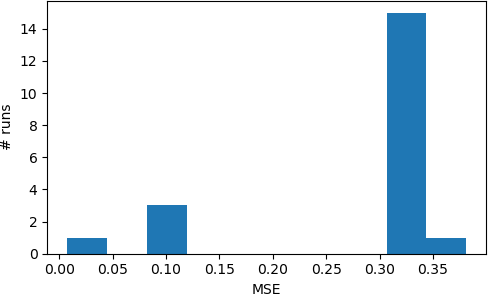
\includegraphics[width=\textwidth]{hist}
         \caption{Histogram of MSE of test batch using ADAM optimizer and 40 data points}
         \label{adamhist}
     \end{subfigure}
     \begin{subfigure}[b]{0.49\textwidth}
         \centering
         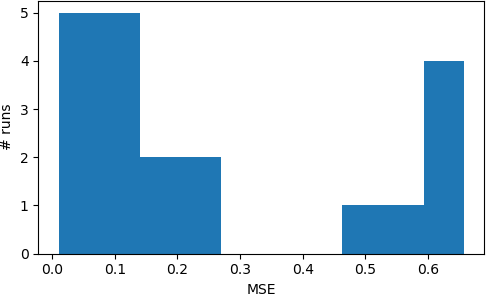
\includegraphics[width=\textwidth]{almhist}
         \caption{Histogram of MSE of test batch using ALM optimizer and 40 data points}
         \label{almhist}
     \end{subfigure}
     \caption{Histograms of MSE batch using 40 data points and ReLU activation function. Both histograms show a bimodal distribution}
     \label{hist}
\end{figure}


The avg MSE, time and epochs has only been calculated over those runs which converged. In the best runs, ADAM typically beats ALM in performance, and could probably even improve further given more epochs. However on average the performance is similar, and ALM converges more often than ADAM. 

The network using ReLU activation function is especially difficult to train, as ADAM only converges 14 times in 60 total runs. In comparison ALM converges 47 times. This may be expected as the main strength of ReLU is found in large networks. In this network the "dying ReLU" problem seems to appear often \cite{Lu2020}. Because the derivative of ReLU is zero for all negative inputs, some nodes may get stuck and receive no gradient updates in a Gradient Descent method such as ADAM. On the other hand, the extra degrees of freedom in the ALM method may allow it to avoid this problem more often.

Another point is that the run time of ALM scales approximately quadratically with the amount of data points N, while the runtime of ADAM stays constant. This is because the size of the Jacobian in ALM scales approximately quadratically with N, see equation \ref{}. In backpropagation the only factor which scales with N is the computation of the loss in the forward pass, which must be executed for every sample. This test has a small dataset, for which the computation of the loss is small compared to the other parts of the ADAM algorithm. In Big Data problems this cost is mitigated by using mini-batches to compute an approximate gradient instead of computing over the whole dataset. This idea could be applied to the ALM method, but this is left for future work.


\section{Santa Fe timeseries data}
In this section the two algorithms are compared for a more practical example. The data in question comes from a competition organised by the Santa Fe Institute \cite{weigend2018time}. It contains 1000 points of experimental data originating from fluctuations in a far-infrared laser. The dynamics can be approximately described by a set of three coupled nonlinear ordinary differential equations. It also contains 100 points of test data for which a prediction must be made. Figure \ref{santafedata} plots the data in its entirety. The test data has been colored orange.

\begin{figure}
   	\centering
	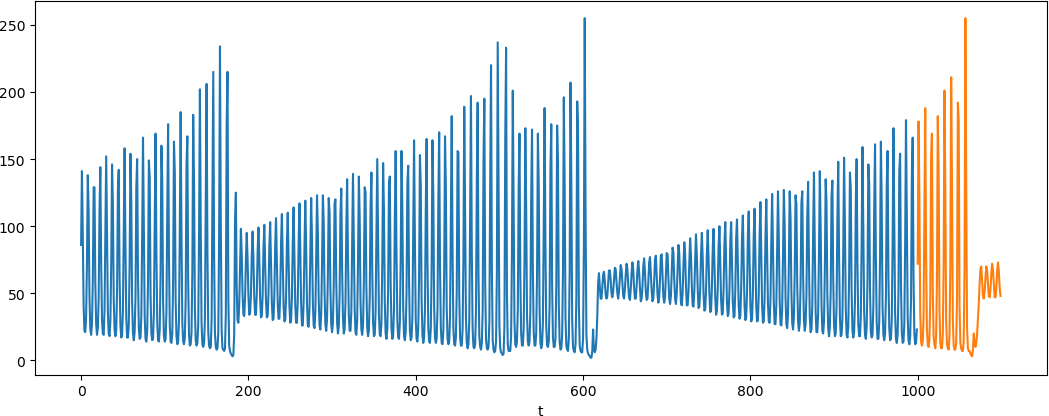
\includegraphics[width=\textwidth]{santafe}
	\caption{Santa Fe timeseries data. The training data has been plotted in blue, the test data in orange.}
	\label{santafedata}
\end{figure}

For this prediction task a recurrent neural network is set up with one hidden layer:

\begin{equation}
\hat{y}_{k+1} = f_W(\begin{bmatrix} \hat{y}_{k} & \hat{y}_{k-1} & ... & \hat{y}_{k-p}\end{bmatrix}^T)
\end{equation}

Each prediction $\hat{y}_{k+1}$ is made based on a vector of the previous $p$ predictions. Once initialized this network can make new predictions by feeding itself previous predictions. It is a network with $p$ inputs, and one output. 

Based on results from \cite{suykens2020}, a network is chosen with 80 inputs and 48 nodes in the hidden layer. The activation function is $\tanh$. The data is first normalized to have a mean of 0 and a standard deviation of 1. Next input-output pairs $(\textbf{x}_i,y_i)$  are generated from the dataset. Because each output data point $y_i$ needs a corresponding vector $\textbf{x}_i$ of 80 previous inputs, the first 80 training points cannot serve as output. This leaves 920 input-output pairs in the dataset. Due to memory limitations, the training set is restricted to 600 pairs, leaving 320 pairs as validation data. The data is randomly distributed over these two sets. Both algorithm are run 4 times, in each run both algorithms start with the same initial weights and dataset distribution. The test is run on an Intel(R) Core(TM) i5-7300HQ CPU @ 2.50GHz with 8Gi RAM and SSD hard disk.

Figure \ref{laserpred} plots the prediction of the best performing run for each algorithm, while figure \ref{laserconv} plots the corresponding training history. The prediction by the network trained by ADAM is better. While both networks predict the large oscillations reasonably well, the reset that happens when the oscillations get too big is only predicted by the network trained by ADAM. Curiously the MSE of the validation set does not improve much during training in either algorithm. The plot of the MSE during training is similar for both algorithms.

Table \ref{rectab} lists the numerical results of the test. The MSE of the training data is similar for both algorithms, but slightly better for ADAM. The MSE of the prediction compared to the test data is much better for ADAM. The biggest difference is in running time, it takes ALM on average 20min to finish a run, while for ADAM it takes 20s. This is because the Jacobian scales quadratically in size with the number of data points. Table \ref{jevaltab} shows the number of calls to the Jacobian per epoch. Most calls are made in the first epochs.

\section{Conclusion}
In this chapter the new algorithm is tested against ADAM, an industry standard backpropagation method.

In the first experiment a small regression problem is selected which is difficult to train for classical gradient descent methods.  In this test ALM converges in 46 out of 60 training runs, while ADAM converges only 14 out of 60 runs. ALM also shows a shorter running time.

In the second experiment a time series prediction problem is selected using the Santa Fe competition laser dataset. A recurrent neural network is trained to predict time series data for this nonlinear system. The prediction made by the network trained by ADAM had an MSE of $9.100e^{-2}$ while the network trained by ALM showed an MSE of $8.288e^{-1}$. Because this problem is much larger in terms of dataset size and network size, ALM took on average 1201s to finish, while ADAM needed 20.9s.

ALM shows promising results, but so far is limited by the size of the dataset. Implementing a mini-batch training mode could address this limitation.





\begin{figure}[p]
     \centering
     \begin{subfigure}[b]{0.49\textwidth}
         \centering
         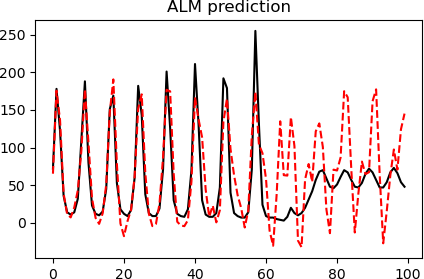
\includegraphics[width=\textwidth]{almpred}
         \caption{Prediction of network trained with ALM}
         \label{almpred}
     \end{subfigure}
     \begin{subfigure}[b]{0.49\textwidth}
         \centering
         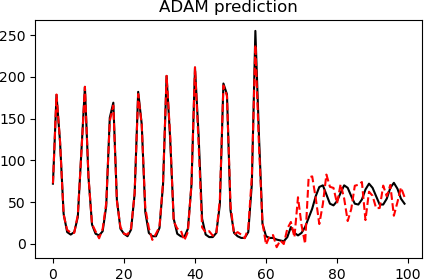
\includegraphics[width=\textwidth]{adampred}
         \caption{Prediction of network trained with ADAM}
         \label{adampred}
     \end{subfigure}
     \caption{Best network prediction compared to test set for both algorithms}
     \label{laserpred}
\end{figure}

\begin{figure}[p]
     \centering
     \begin{subfigure}[b]{0.49\textwidth}
         \centering
         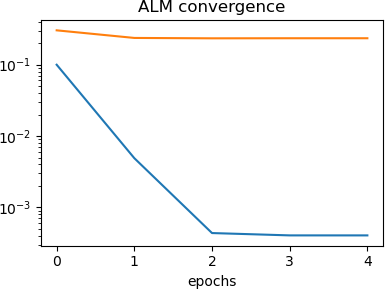
\includegraphics[width=\textwidth]{almlaserconv}
         \caption{Training and validation MSE for ALM}
         \label{almlaserconv}
     \end{subfigure}
     \begin{subfigure}[b]{0.49\textwidth}
         \centering
         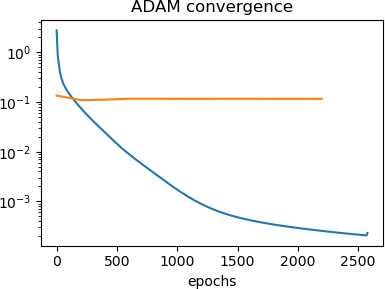
\includegraphics[width=\textwidth]{adamlaserconv}
         \caption{Training and validation MSE for ADAM}
         \label{adamlaserconv}
     \end{subfigure}
     \caption{Comparison of convergence behaviour on training set and validation set for both algorithms.}
     \label{laserconv}
\end{figure}

\begin{table}
\renewcommand{\arraystretch}{1.3}
\centering
\small
\makebox[\textwidth][c]{
\begin{tabular}{r| c c c c c c }
	Algo & avg MSE          & best MSE         & avg pred MSE     & best pred MSE    & epochs   & time \\ \hline
     ALM & $ 3.712e^{-4} $ & $ 2.779e^{-4} $ & $ 1.070e^0    $ & $ 8.288e^{-1} $ & $ 5    $ & 1201s \\
    ADAM & $ 2.517e^{-4} $ & $ 2.329e^{-4} $ & $ 2.016e^{-1} $ & $ 9.100e^{-2} $ & $ 2353 $ & 20.9s
\end{tabular}
}
\caption{Results of training a recurrent neural network}
\label{rectab}
\end{table}


\begin{table}
\centering
\begin{tabular}{r| c c c c c }
Epoch	 	& 1	& 2 & 3 & 4 & 5 \\ \hline
\#evals & 42.25 & 12.75 & 17.0  &   3.0  &    2.0 \\
\end{tabular}
\caption{Average number of Jacobian evaluations per epoch}
\label{jevaltab}
\end{table}





%\begin{figure}[p]
%         \centering
%         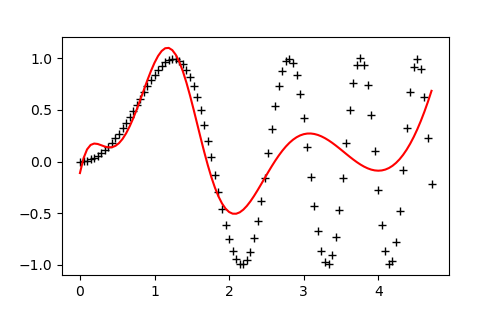
\includegraphics[width=\textwidth]{sine_squared}
%         \caption{Feedforward network with 2 hidden layers of 20 relu units, trained on test function using ALM, using 80 training pairs}
%\end{figure}



%%% Local Variables: 
%%% mode: latex
%%% TeX-master: "thesis"
%%% End: 
